% !Rnw weave = knitr

%%%%%%%%%%%%%%%%%%%%%%%%%%%%%%%%%%%%%%%%%%%%%%%%%%%%%%%%%%%%%%%%%%%%%%%%%%
%%%%%%%%%%%%%%%%%%%%%%%%%%%%%%%%%%%%%%%%%%%%%%%%%%%%%%%%%%%%%%%%%%%%%%%%%%

% Preambuła TeX-a. Można dodać brakujące pakiety w razie potrzeby

\documentclass[12pt, a4paper]{article}\usepackage[]{graphicx}\usepackage[]{xcolor}
% maxwidth is the original width if it is less than linewidth
% otherwise use linewidth (to make sure the graphics do not exceed the margin)
\makeatletter
\def\maxwidth{ %
  \ifdim\Gin@nat@width>\linewidth
    \linewidth
  \else
    \Gin@nat@width
  \fi
}
\makeatother

\definecolor{fgcolor}{rgb}{0.345, 0.345, 0.345}
\newcommand{\hlnum}[1]{\textcolor[rgb]{0.686,0.059,0.569}{#1}}%
\newcommand{\hlstr}[1]{\textcolor[rgb]{0.192,0.494,0.8}{#1}}%
\newcommand{\hlcom}[1]{\textcolor[rgb]{0.678,0.584,0.686}{\textit{#1}}}%
\newcommand{\hlopt}[1]{\textcolor[rgb]{0,0,0}{#1}}%
\newcommand{\hlstd}[1]{\textcolor[rgb]{0.345,0.345,0.345}{#1}}%
\newcommand{\hlkwa}[1]{\textcolor[rgb]{0.161,0.373,0.58}{\textbf{#1}}}%
\newcommand{\hlkwb}[1]{\textcolor[rgb]{0.69,0.353,0.396}{#1}}%
\newcommand{\hlkwc}[1]{\textcolor[rgb]{0.333,0.667,0.333}{#1}}%
\newcommand{\hlkwd}[1]{\textcolor[rgb]{0.737,0.353,0.396}{\textbf{#1}}}%
\let\hlipl\hlkwb

\usepackage{framed}
\makeatletter
\newenvironment{kframe}{%
 \def\at@end@of@kframe{}%
 \ifinner\ifhmode%
  \def\at@end@of@kframe{\end{minipage}}%
  \begin{minipage}{\columnwidth}%
 \fi\fi%
 \def\FrameCommand##1{\hskip\@totalleftmargin \hskip-\fboxsep
 \colorbox{shadecolor}{##1}\hskip-\fboxsep
     % There is no \\@totalrightmargin, so:
     \hskip-\linewidth \hskip-\@totalleftmargin \hskip\columnwidth}%
 \MakeFramed {\advance\hsize-\width
   \@totalleftmargin\z@ \linewidth\hsize
   \@setminipage}}%
 {\par\unskip\endMakeFramed%
 \at@end@of@kframe}
\makeatother

\definecolor{shadecolor}{rgb}{.97, .97, .97}
\definecolor{messagecolor}{rgb}{0, 0, 0}
\definecolor{warningcolor}{rgb}{1, 0, 1}
\definecolor{errorcolor}{rgb}{1, 0, 0}
\newenvironment{knitrout}{}{} % an empty environment to be redefined in TeX

\usepackage{alltt}
\usepackage[T1]{fontenc}
\usepackage{graphicx}
\usepackage{float}
\usepackage[colorlinks=true, linkcolor=blue]{hyperref}
\usepackage{amsmath, amsthm, amssymb, amscd}
\usepackage{enumerate}
\usepackage{polski}
\usepackage{float}
\newtheorem{thm}{Twierdzenie}
\newtheorem{lem}{Lemat}
\newtheorem{cor}{Wniosek}
\newtheorem{prop}{Propozycja}
\newtheorem{rem}{Uwaga}
\newtheorem{note}{Notka}
\newtheorem{fact}{Fakt}
\newtheorem{defn}{Definicja}
\counterwithin{equation}{section}
\def \E {\mathbb{E}}
\def \P {\mathbb{P}}
%%%%%%%%%%%%%%%%%%%%%%%%%%%%%%%%%%%%%%%%%%%%%%%%%%%%%%%%%%%%%%%%%%%%%%%%%%
%%%%%%%%%%%%%%%%%%%%%%%%%%%%%%%%%%%%%%%%%%%%%%%%%%%%%%%%%%%%%%%%%%%%%%%%%%
%NIE ZMIENIAĆ!
\usepackage[top=2.5cm, bottom=2.5cm, left=2cm, right=2cm]{geometry}
\makeatletter
\newcommand\numerraportu[1]{\renewcommand\@title{}}
\renewcommand{\maketitle}{
    \begin{center}
        \vspace{5pt}
        \textbf{\Huge \sffamily Konstrukcja generatorów liczb losowych i symulacyjna analiza ich własności}\\
        \vspace{15pt}
        \textbf{\Large \sffamily \@title}\\
        \vspace{10pt}
        {\Large \sffamily \@author}\\
        \vspace{10pt}
        \hrulefill\\
        \vspace{20pt}
    \end{center}
}
\usepackage{fancyhdr}
\pagestyle{fancy}
\fancyhf{}
\fancyhead[R]{\thepage}
\fancyhead[L]{\@author}
\setlength{\headsep}{10pt}
\makeatother
%%%%%%%%%%%%%%%%%%%%%%%%%%%%%%%%%%%%%%%%%%%%%%%%%%%%%%%%%%%%%%%%
%%%%%%%%%%%%%%%%%%%%%%%%%%%%%%%%%%%%%%%%%%%%%%%%%%%%%%%%%%%%%%%%


% Dane raportu - wypełniają studenci

\author{Stanisław Olek}
\numerraportu{1}


%%%%%%%%%%%%%%%%%%%%%%%%%%%%%%%%%%%%%%%%%%%%%%%%%%%%%%%%%%%%%%%%
%%%%%%%%%%%%%%%%%%%%%%%%%%%%%%%%%%%%%%%%%%%%%%%%%%%%%%%%%%%%%%%%

\IfFileExists{upquote.sty}{\usepackage{upquote}}{}
\begin{document}

%Poniżej chunk z kodem. Ponieważ tu są ustawienia globalne, np. pobierane biblioteki, nie chcemy by kod był wyświetlany w pliku PDF, więc wybieramy opcję echo=FALSE. Dla opcji echo=TRUE chunk z kodem będzie wyświetlany w pliku PDF. Jest też opcja eval, jeżeli ma wartość TRUE (domyślna), to kod z chunka będzie wykonywany a wynik zostanie zapisany w sesji R. Jeżeli ma wartość False, to kod z chunka nie będzie wykonywany a jedynie sprawdzany pod kątem poprawności.

%Przed pierwszą kompilacją oba pakiety knitr i xtable muszą być zainstalowane przy pomocy komendy install.packages('nazwa pakietu') wywołanej w konsoli.

%Strona tytułowa i spis treści
\maketitle

\tableofcontents
\thispagestyle{plain}

%%%%%%%%%%%%%%%%%%%%%%%%%%%%%%%%%%%%%%%%%%%%%%%%%%%%%%%%%%%%%%%%%%%%%%%%%%
%%%%%%%%%%%%%%%%%%%%%%%%%%%%%%%%%%%%%%%%%%%%%%%%%%%%%%%%%%%%%%%%%%%%%%%%%%
\newpage
\section{Problem 1 -- Generator kongruencyjny}
\begin{itemize}
\item Zaimplementuj liniowy generator kongruencyjny liczb pseudolosowych $x_1, x_2,\ldots$:
$$(s_0=1)\quad s_n=as_{n-1}\; {\rm mod} \; m;\quad x_n=s_n/m,\quad n=1,2,\ldots, \mbox{gdzie}$$
\begin{enumerate}
\item[i] $m=37$, $a=19$,
\item[ii] $m=2^{31}-1$, $a=39373$.
\end{enumerate} 
\item Sprawdź empirycznie, jaki okres ma pierwszy z tych generatorów.
\item Narysuj $50$ kolejnych liczb pseudolosowych j.w. jako punkty na odcinku jednostkowym. Narysuj histogram. Skomentuj rysunek.
\item Narysuj $50$ kolejnych par liczb pseudolosowych j.w. jako punkty na kwadracie jednostkowym. Skomentuj rysunek.
\end{itemize}

\medskip

\noindent{\large\bf \sffamily Rozwiązanie:}
\vspace{15pt}
%%%%%%%%%%%%%%%%%%%%%%%%%%%%%%%%%%%%%%%%%%%%%%%%%%%%%%%%%%%%%%%%%%%%%%%%%%
%%%%%%%%%%%%%%%%%%%%%%%%%%%%%%%%%%%%%%%%%%%%%%%%%%%%%%%%%%%%%%%%%%%%%%%%%%

\begin{itemize}
\item

\begin{knitrout}
\definecolor{shadecolor}{rgb}{0.969, 0.969, 0.969}\color{fgcolor}\begin{kframe}
\begin{alltt}
\hlstd{generator_kongruencyjny} \hlkwb{<-} \hlkwa{function}\hlstd{(}\hlkwc{a}\hlstd{,} \hlkwc{m}\hlstd{,} \hlkwc{n}\hlstd{) \{}
  \hlstd{s_n} \hlkwb{=} \hlkwd{c}\hlstd{(}\hlnum{1}\hlstd{)}
  \hlkwa{for} \hlstd{(i} \hlkwa{in} \hlnum{1}\hlopt{:}\hlstd{n) \{}
    \hlstd{k} \hlkwb{<-} \hlstd{s_n[}\hlkwd{length}\hlstd{(s_n)]}
    \hlstd{s_n} \hlkwb{<-} \hlkwd{c}\hlstd{(s_n, (a} \hlopt{*} \hlstd{k)} \hlopt \hlstd{m)}
  \hlstd{\}}
  \hlstd{x_n} \hlkwb{<-} \hlstd{s_n} \hlopt{/} \hlstd{m}
  \hlkwd{return}\hlstd{(x_n[}\hlopt{-}\hlnum{1}\hlstd{])}
\hlstd{\}}
\end{alltt}
\end{kframe}
\end{knitrout}


\begin{description}
\item[i] $m = 37, a=19$
\begin{knitrout}
\definecolor{shadecolor}{rgb}{0.969, 0.969, 0.969}\color{fgcolor}\begin{kframe}
\begin{verbatim}
##  [1] 0.51351351 0.75675676 0.37837838 0.18918919 0.59459459 0.29729730
##  [7] 0.64864865 0.32432432 0.16216216 0.08108108 0.54054054 0.27027027
## [13] 0.13513514 0.56756757 0.78378378 0.89189189 0.94594595 0.97297297
## [19] 0.48648649 0.24324324 0.62162162 0.81081081 0.40540541 0.70270270
## [25] 0.35135135 0.67567568 0.83783784 0.91891892 0.45945946 0.72972973
## [31] 0.86486486 0.43243243 0.21621622 0.10810811 0.05405405 0.02702703
## [37] 0.51351351 0.75675676 0.37837838 0.18918919 0.59459459 0.29729730
## [43] 0.64864865 0.32432432 0.16216216 0.08108108 0.54054054 0.27027027
## [49] 0.13513514 0.56756757
\end{verbatim}
\end{kframe}
\end{knitrout}


\item[ii] $m = 2^{31}-1, a=39373$
\begin{knitrout}
\definecolor{shadecolor}{rgb}{0.969, 0.969, 0.969}\color{fgcolor}\begin{kframe}
\begin{verbatim}
##  [1] 1.833448e-05 7.218836e-01 7.212037e-01 9.520167e-01 7.553457e-01
##  [6] 2.248237e-01 9.826929e-01 5.675375e-01 6.550636e-01 8.177157e-01
## [11] 9.210877e-01 9.843399e-01 4.165816e-01 6.655500e-02 4.699210e-01
## [16] 2.001585e-01 8.421137e-01 5.425512e-01 8.698889e-01 1.365497e-01
## [21] 3.718927e-01 5.299994e-01 6.661485e-01 2.644647e-01 7.689364e-01
## [26] 3.318948e-01 6.932724e-01 2.146284e-01 5.649799e-01 9.547553e-01
## [31] 5.812586e-01 8.954412e-01 2.078554e-01 8.923246e-01 4.948566e-01
## [36] 9.879381e-01 8.505122e-02 7.217564e-01 7.158718e-01 1.966913e-02
## [41] 4.328017e-01 7.011114e-01 8.611099e-01 4.784881e-01 5.107689e-01
## [46] 5.052171e-01 9.129803e-01 7.747585e-01 5.649881e-01 2.777356e-01
\end{verbatim}
\end{kframe}
\end{knitrout}
\end{description}


\item
\begin{knitrout}
\definecolor{shadecolor}{rgb}{0.969, 0.969, 0.969}\color{fgcolor}\begin{kframe}
\begin{alltt}
\hlstd{okres} \hlkwb{<-} \hlkwa{function}\hlstd{(}\hlkwc{a}\hlstd{,} \hlkwc{m}\hlstd{) \{}
  \hlstd{s_n} \hlkwb{=} \hlnum{1}
  \hlstd{wygenerowane} \hlkwb{=} \hlkwd{c}\hlstd{(s_n)}
  \hlstd{okres} \hlkwb{=} \hlnum{1}
  \hlkwa{while}\hlstd{(}\hlnum{TRUE}\hlstd{) \{}
    \hlstd{s_n} \hlkwb{<-} \hlstd{(a} \hlopt{*} \hlstd{s_n)} \hlopt \hlstd{m}
    \hlkwa{if}\hlstd{(s_n} \hlopt \hlstd{wygenerowane) \{}
      \hlkwa{break}
    \hlstd{\}} \hlkwa{else} \hlstd{\{}
      \hlstd{wygenerowane} \hlkwb{<-} \hlkwd{c}\hlstd{(wygenerowane, s_n)}
      \hlstd{okres} \hlkwb{<-} \hlstd{okres} \hlopt{+} \hlnum{1}
    \hlstd{\}}
  \hlstd{\}}
  \hlkwd{return}\hlstd{(okres)}
\hlstd{\}}
\end{alltt}
\end{kframe}
\end{knitrout}

\begin{knitrout}
\definecolor{shadecolor}{rgb}{0.969, 0.969, 0.969}\color{fgcolor}\begin{kframe}
\begin{verbatim}
## Okres pierwszego generatora: 36
\end{verbatim}
\end{kframe}
\end{knitrout}

\break
\item
\begin{minipage}{\linewidth}
\begin{knitrout}
\definecolor{shadecolor}{rgb}{0.969, 0.969, 0.969}\color{fgcolor}

{\centering 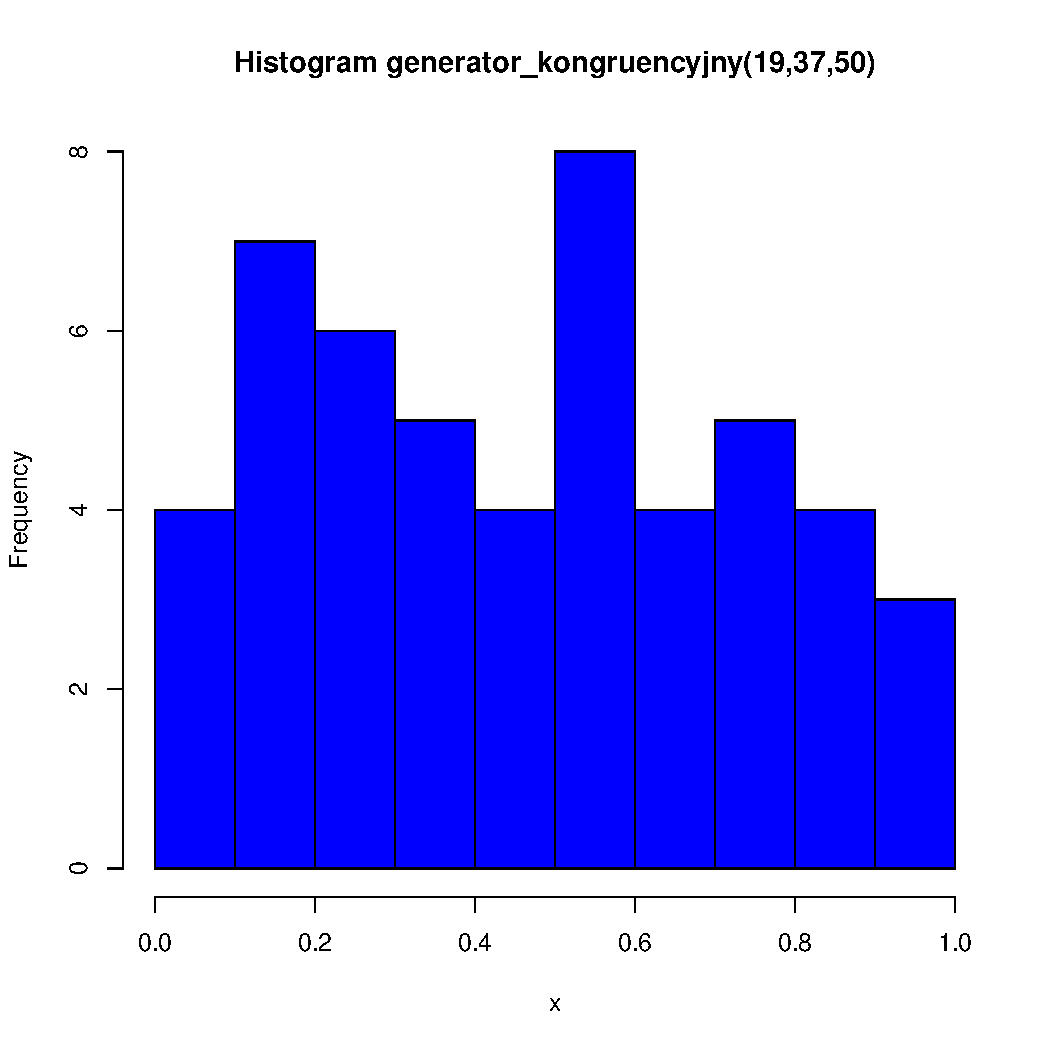
\includegraphics[width=\maxwidth]{figure/unnamed-chunk-4-1} 

}


\end{knitrout}
\end{minipage}
Jeśli spojrzymy na histogram to wydaje się, że dane nie są idealnie równomiernie rozłożone, ponieważ liczba wystąpień w poszczególnych przedziałach różni się.
Najwięcej obserwacji znajduje się w przedziale od 0.5 do 0.6, gdzie mamy 8 wystąpień. Najmniej obserwacji jest w ostatnim przedziale od 0.9 do 1.0, gdzie mamy tylko 3 wystąpienia. Pozostałe przedziały mają liczbę wystąpień między 4 a 7.
Taki rozkład może sugerować, że dane nie są idealnie równomiernie rozłożone, ale nie ma też bardzo dużych odchyleń od równomierności.


\begin{knitrout}
\definecolor{shadecolor}{rgb}{0.969, 0.969, 0.969}\color{fgcolor}

{\centering 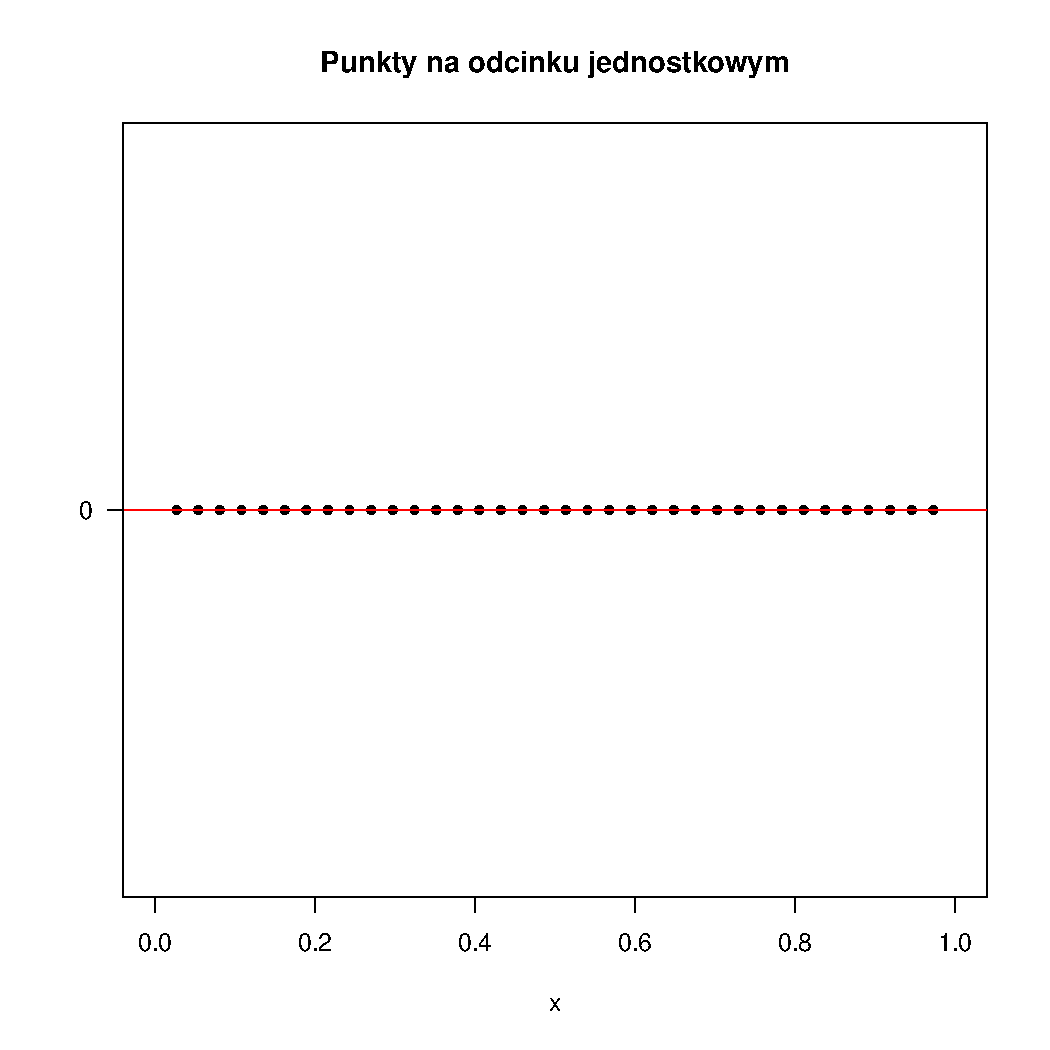
\includegraphics[width=\maxwidth]{figure/unnamed-chunk-5-1} 

}


\end{knitrout}
Jeśli spojrzymy na rozkład punktów na odcinku jednostkowym, możemy zauważyć, że liczby pseudolosowe wydają się być stosunkowo równomiernie rozłożone bez widocznych wzorców lub skupisk, pomimo że wartości m i a są stosunkowo małe.


\break
\item 
\begin{minipage}{\linewidth}
\begin{knitrout}
\definecolor{shadecolor}{rgb}{0.969, 0.969, 0.969}\color{fgcolor}

{\centering 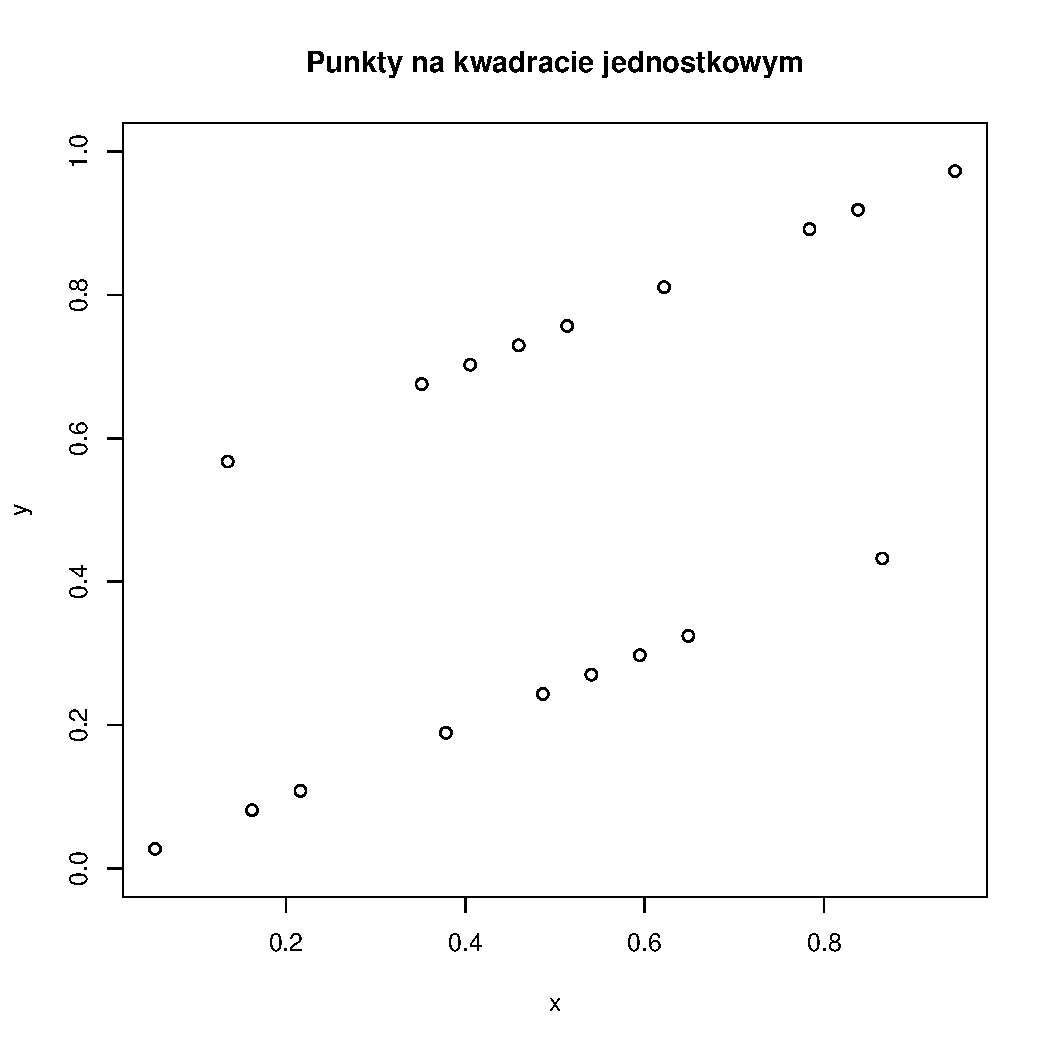
\includegraphics[width=\maxwidth]{figure/unnamed-chunk-6-1} 

}


\end{knitrout}
\end{minipage}

Z uwagi na charakterystykę liniowych generatorów kongruentnych i małą wartość m punkty wykazują wyraźną regularność - układają się w linie. Świadczy to o tym, że liczby nie są równomiernie rozłożona na kwadracie, co jest typową cechą dla generatorów kongruentnych i małych wartości parametrów.


\end{itemize}

%%%%%%%%%%%%%%%%%%%%%%%%%%%%%%%%%%%%%%%%%%%%%%%%%%%%%%%%%%%%%%%%%%%%%%%%%%
%%%%%%%%%%%%%%%%%%%%%%%%%%%%%%%%%%%%%%%%%%%%%%%%%%%%%%%%%%%%%%%%%%%%%%%%%%
\newpage
\section{Problem 2 -- Generator standardowy w R}

\begin{itemize}
\item Narysuj $50$ kolejnych par liczb pseudolosowych jako punkty na kwadracie jednostkowym dla standardowego generatora zaimplementowanego w pakiecie R. 
\item Czy otrzymane pary liczb pseudolosowych mają rozkład jednostajny na kwadracie $[0,1]^2$? Zaproponuj, jak to weryfikować. W jaki sposób ta własność łączy się z własnością niezależności kolejnych liczb?
\item Jak inicjować obliczenia, żeby za każdym razem otrzymywać ten sam ciąg $50$-ciu par? Czy taka powtarzalność (replikowalność) jest sprzeczna z ideą symulacji pseudolosowych?
 \end{itemize}

\medskip

\noindent{\large\bf \sffamily Rozwiązanie:}
\vspace{15pt}
%%%%%%%%%%%%%%%%%%%%%%%%%%%%%%%%%%%%%%%%%%%%%%%%%%%%%%%%%%%%%%%%%%%%%%%%%%
%%%%%%%%%%%%%%%%%%%%%%%%%%%%%%%%%%%%%%%%%%%%%%%%%%%%%%%%%%%%%%%%%%%%%%%%%%
\begin{itemize}
\item
\begin{minipage}{\linewidth}
\begin{knitrout}
\definecolor{shadecolor}{rgb}{0.969, 0.969, 0.969}\color{fgcolor}

{\centering 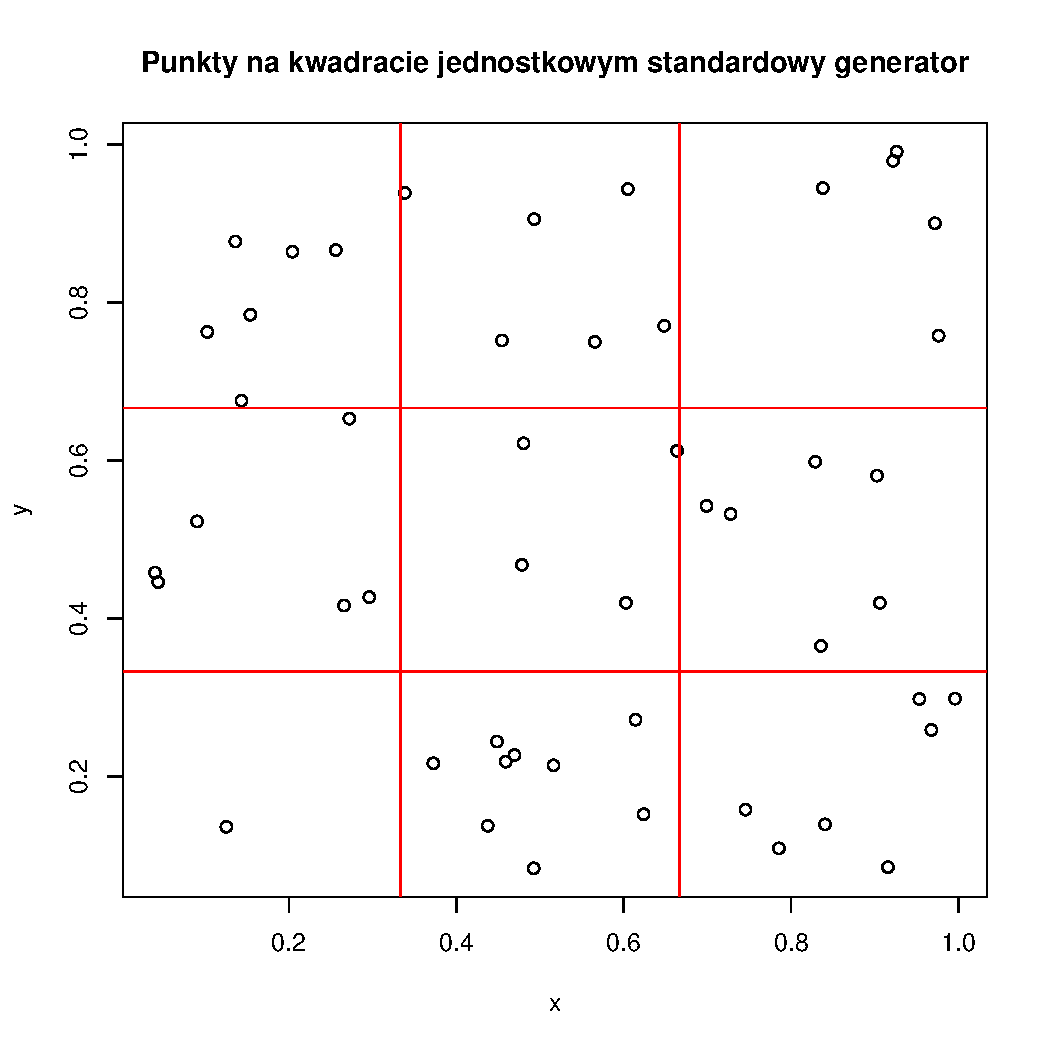
\includegraphics[width=\maxwidth]{figure/unnamed-chunk-7-1} 

}


\end{knitrout}
\end{minipage}


Tak, jeśli używamy funkcji \textbf{runif()}, otrzymujemy liczby pseudolosowe, które mają rozkład jednostajny na przedziale od 0 do 1. Kiedy generujemy pary takich liczb, zakładamy, że każda para jest punktem na kwadracie jednostkowym $[0, 1]^{2}$, gdzie każdy punkt ma taką samą szansę na pojawienie się w dowolnym miejscu na tym kwadracie.
Aby zweryfikować, czy otrzymane pary liczb pseudolosowych mają rozkład jednostajny, można przeprowadzić test statystyczny, na przykład test chi-kwadrat Pearsona. Test ten pozwala sprawdzić, czy obserwowane częstości punktów w różnych obszarach kwadratu jednostkowego są zgodne z oczekiwaniami dla rozkładu jednostajnego.

Oto przykładowy sposób weryfikacji:
\begin{enumerate}
  \item Podziel kwadrat jednostkowy na mniejsze, równomierne kwadraty (na przykład 3x3, co daje 9 mniejszych kwadratów).
  \item Policz, ile punktów wpada do każdego z mniejszych kwadratów.
  \item Porównaj obserwowane liczby z oczekiwanymi liczbami dla rozkładu jednostajnego.
  \item Użyj testu chi-kwadrat do obliczenia p-wartości i zdecyduj, czy odrzucić hipotezę zerową o rozkładzie jednostajnym.
\end{enumerate}

Własność niezależności kolejnych liczb w generatorze liczb pseudolosowych jest ważna, ponieważ oznacza, że każda liczba jest generowana bez wpływu na poprzednie liczby. Dla rozkładu jednostajnego na kwadracie jednostkowym oznacza to, że położenie jednego punktu nie wpływa na położenie kolejnego. Jeśli liczby nie byłyby niezależne, moglibyśmy zauważyć wzorce lub "skupiska" punktów na kwadracie, co wskazywałoby na problem z generatorem liczb pseudolosowych.


\break

\item
Aby za każdym razem otrzymywać ten sam ciąg 50-ciu par liczb pseudolosowych, należy zainicjować generator liczb pseudolosowych tym samym "ziarnem", wykorzystując komendę:
\begin{knitrout}
\definecolor{shadecolor}{rgb}{0.969, 0.969, 0.969}\color{fgcolor}\begin{kframe}
\begin{alltt}
\hlkwd{set.seed}\hlstd{(n)}
\end{alltt}
\end{kframe}
\end{knitrout}
gdzie \textbf{n} jest pewną liczbą naturalną.

\item
Powtarzalność nie jest sprzeczna z ideą symulacji pseudolosowych. Wręcz przeciwnie, jest to jedna z pożądanych cech generatorów liczb pseudolosowych. Generatory liczb pseudolosowych są deterministyczne, co oznacza, że dla tego samego ziarna zawsze wygenerują ten sam ciąg liczb. To pozwala na replikację eksperymentów i testów.
Idea symulacji pseudolosowych polega na tym, że choć liczby generowane przez te algorytmy są deterministyczne (i w tym sensie nie są "prawdziwie" losowe), ich właściwości statystyczne sprawiają, że w wielu zastosowaniach są one wystarczająco "dobre" do naśladowania losowości.

\end{itemize}


\newpage
\section{Problem 3 -- Symulacja dyskretnych zmiennych losowych}

\begin{itemize}
\item Napisz generator liczb losowych o rozkładzie dwupunktowym: $\mathbb P(X=1)=p$, $\mathbb P(X=0)=1-p$, gdzie $p\in [0,1]$.

\item Napisz generator liczb losowych dla rozkładu dwumianowego. Narysuj histogram dla próby (prostej) z tego rozkładu.

\item Napisz generator dla rozkładu Poissona. Wykonaj odręcznie obliczenia przygotowawcze. 
Działanie generatora sprawdź poprzez analizę histogramów lub w inny sposób.
\end{itemize}

\medskip

\noindent{\large\bf \sffamily Rozwiązanie:}
\vspace{15pt}
%%%%%%%%%%%%%%%%%%%%%%%%%%%%%%%%%%%%%%%%%%%%%%%%%%%%%%%%%%%%%%%%%%%%%%%%%%
%%%%%%%%%%%%%%%%%%%%%%%%%%%%%%%%%%%%%%%%%%%%%%%%%%%%%%%%%%%%%%%%%%%%%%%%%%

\begin{itemize}

\item
\begin{knitrout}
\definecolor{shadecolor}{rgb}{0.969, 0.969, 0.969}\color{fgcolor}\begin{kframe}
\begin{alltt}
\hlstd{gen_0_1} \hlkwb{<-} \hlkwa{function}\hlstd{(}\hlkwc{p}\hlstd{) \{}
  \hlstd{x} \hlkwb{<-} \hlkwd{runif}\hlstd{(}\hlnum{1}\hlstd{)}
  \hlkwa{if}\hlstd{(x} \hlopt{<=} \hlstd{p)\{}
    \hlkwd{return}\hlstd{(}\hlnum{1}\hlstd{)}
  \hlstd{\}}
  \hlkwa{else}\hlstd{\{}
    \hlkwd{return}\hlstd{(}\hlnum{0}\hlstd{)}
  \hlstd{\}}
\hlstd{\}}

\hlstd{generator_dwupunktowy} \hlkwb{<-} \hlkwa{function}\hlstd{(}\hlkwc{n}\hlstd{,}\hlkwc{p}\hlstd{)\{}
  \hlstd{x} \hlkwb{<-} \hlkwd{c}\hlstd{(}\hlnum{1}\hlstd{)}
  \hlkwa{for} \hlstd{(i} \hlkwa{in} \hlnum{1}\hlopt{:}\hlstd{n)}
    \hlstd{x[i]} \hlkwb{<-} \hlkwd{gen_0_1}\hlstd{(p)}
  \hlkwd{return}\hlstd{(x)}
\hlstd{\}}
\end{alltt}
\end{kframe}
\end{knitrout}

\item
\begin{knitrout}
\definecolor{shadecolor}{rgb}{0.969, 0.969, 0.969}\color{fgcolor}\begin{kframe}
\begin{alltt}
\hlstd{generator_dwumianowy} \hlkwb{<-} \hlkwa{function}\hlstd{(}\hlkwc{n}\hlstd{,} \hlkwc{m}\hlstd{,} \hlkwc{p}\hlstd{) \{}
  \hlstd{x} \hlkwb{<-} \hlkwd{c}\hlstd{(}\hlnum{1}\hlstd{)}
  \hlkwa{for} \hlstd{(i} \hlkwa{in} \hlnum{1}\hlopt{:}\hlstd{n) \{}
    \hlstd{u} \hlkwb{=} \hlkwd{runif}\hlstd{(m);}
    \hlstd{b} \hlkwb{=} \hlstd{(u} \hlopt{<} \hlstd{p);}
    \hlstd{x[i]} \hlkwb{=} \hlkwd{sum}\hlstd{(b)}
  \hlstd{\}}
  \hlkwd{return}\hlstd{(x)}
\hlstd{\}}
\end{alltt}
\end{kframe}
\end{knitrout}

\break
Generator rozkładu dwumianowego dla parametrów: $n=100, m=10, p=\frac{1}{2}$
\begin{knitrout}
\definecolor{shadecolor}{rgb}{0.969, 0.969, 0.969}\color{fgcolor}

{\centering 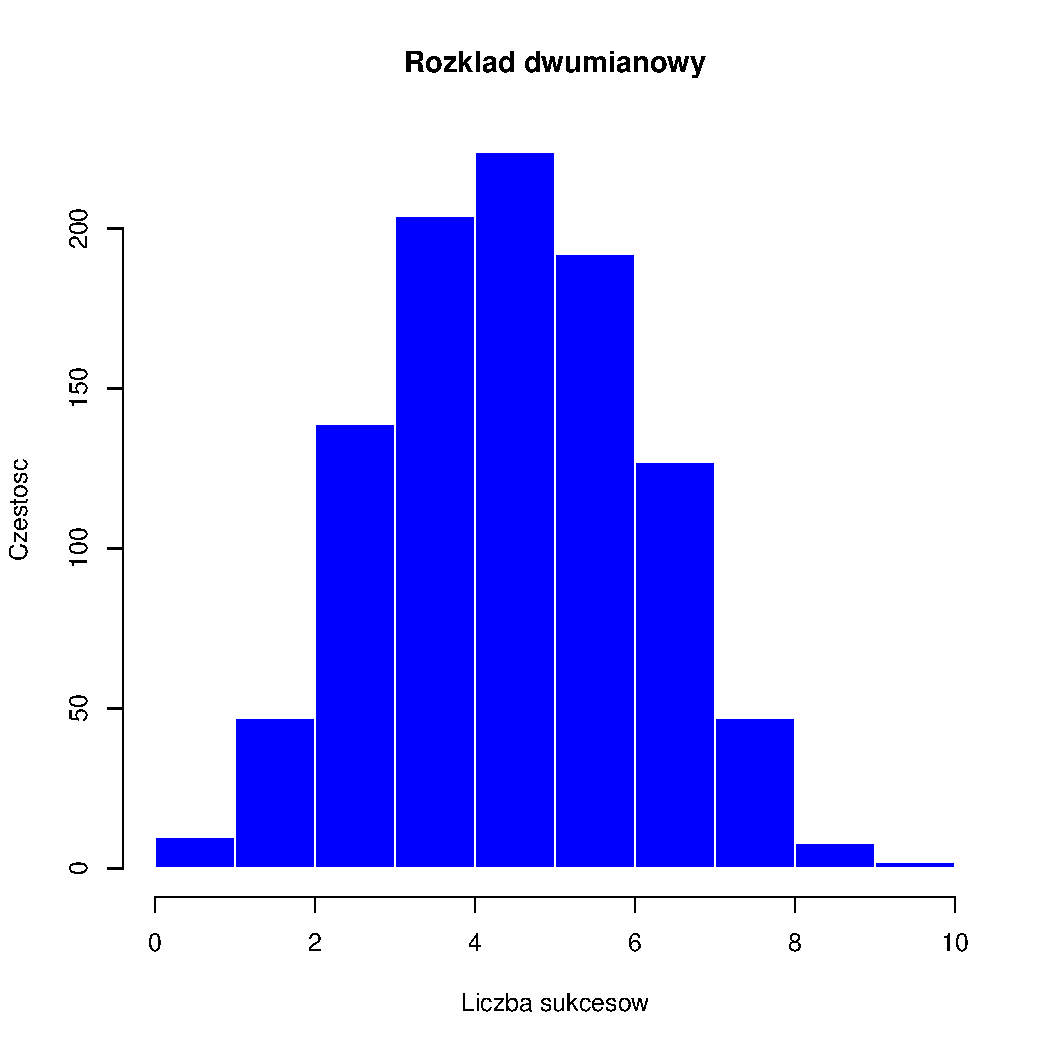
\includegraphics[width=\maxwidth]{figure/unnamed-chunk-9-1} 

}


\end{knitrout}

\item
Generator rozkładu Poissona dla parametrów: $n=100, \lambda=5$
\begin{knitrout}
\definecolor{shadecolor}{rgb}{0.969, 0.969, 0.969}\color{fgcolor}\begin{kframe}
\begin{alltt}
\hlstd{generator_poissona} \hlkwb{<-} \hlkwa{function}\hlstd{(}\hlkwc{n}\hlstd{,}\hlkwc{lambda}\hlstd{) \{}
  \hlstd{tab} \hlkwb{<-} \hlkwd{c}\hlstd{(}\hlnum{0}\hlstd{)}
  \hlkwa{for}\hlstd{(i} \hlkwa{in} \hlnum{1}\hlopt{:}\hlstd{n)\{}
    \hlstd{L} \hlkwb{<-} \hlkwd{exp}\hlstd{(}\hlopt{-}\hlstd{lambda)}
    \hlstd{k} \hlkwb{<-} \hlnum{0}
    \hlstd{iloczyn_p} \hlkwb{<-} \hlnum{1}
    \hlkwa{while}\hlstd{(}\hlnum{TRUE}\hlstd{) \{}
      \hlstd{u} \hlkwb{<-} \hlkwd{runif}\hlstd{(}\hlnum{1}\hlstd{)}
      \hlstd{iloczyn_p} \hlkwb{<-} \hlstd{iloczyn_p} \hlopt{*} \hlstd{u}
      \hlkwa{if}\hlstd{(iloczyn_p} \hlopt{>=} \hlstd{L)\{}
        \hlstd{k} \hlkwb{<-} \hlstd{k} \hlopt{+} \hlnum{1}
      \hlstd{\}} \hlkwa{else}\hlstd{\{}
        \hlstd{tab[i]} \hlkwb{<-} \hlstd{k}
        \hlkwa{break}
      \hlstd{\}}
    \hlstd{\}}
  \hlstd{\}}
  \hlkwd{return}\hlstd{(tab)}
\hlstd{\}}
\end{alltt}
\end{kframe}
\end{knitrout}

\begin{knitrout}
\definecolor{shadecolor}{rgb}{0.969, 0.969, 0.969}\color{fgcolor}

{\centering 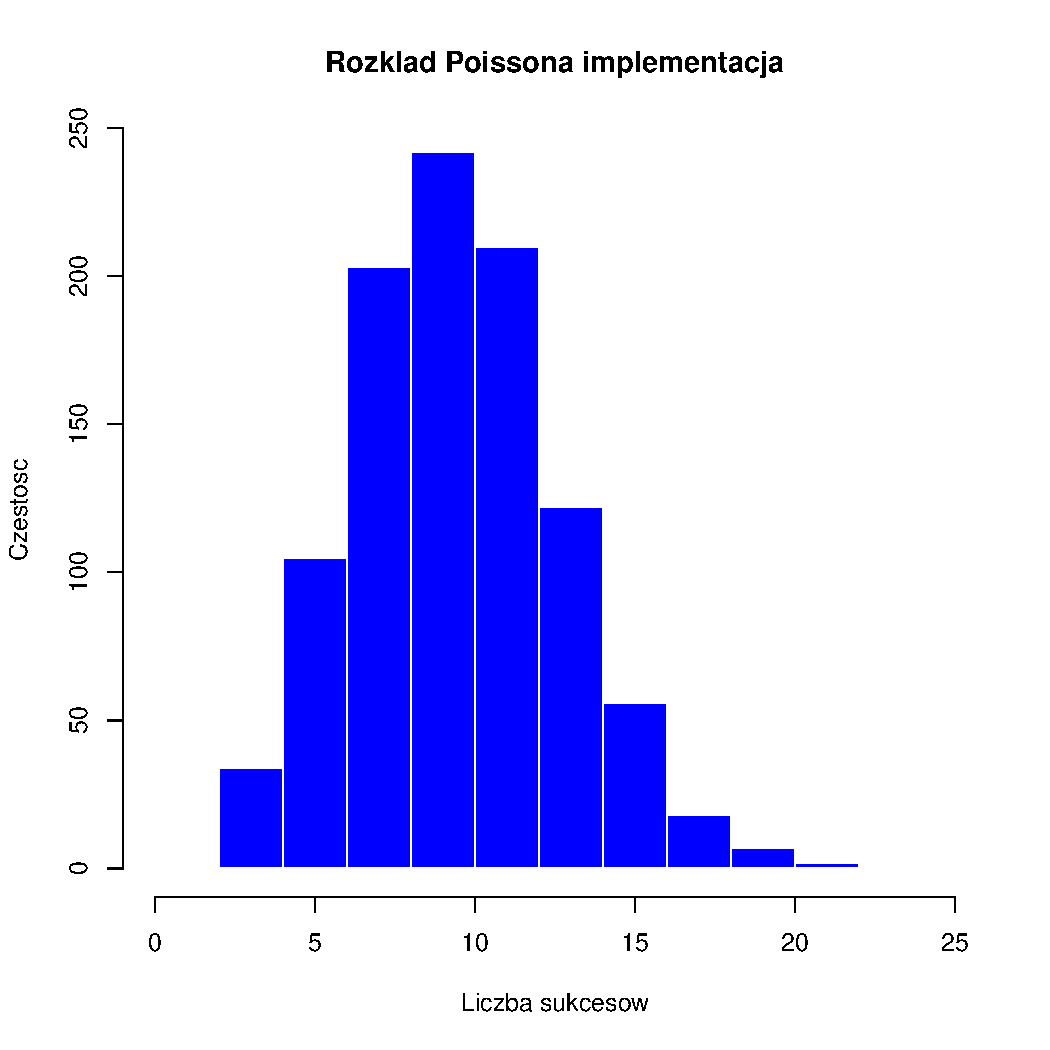
\includegraphics[width=\maxwidth]{figure/unnamed-chunk-10-1} 

}




{\centering 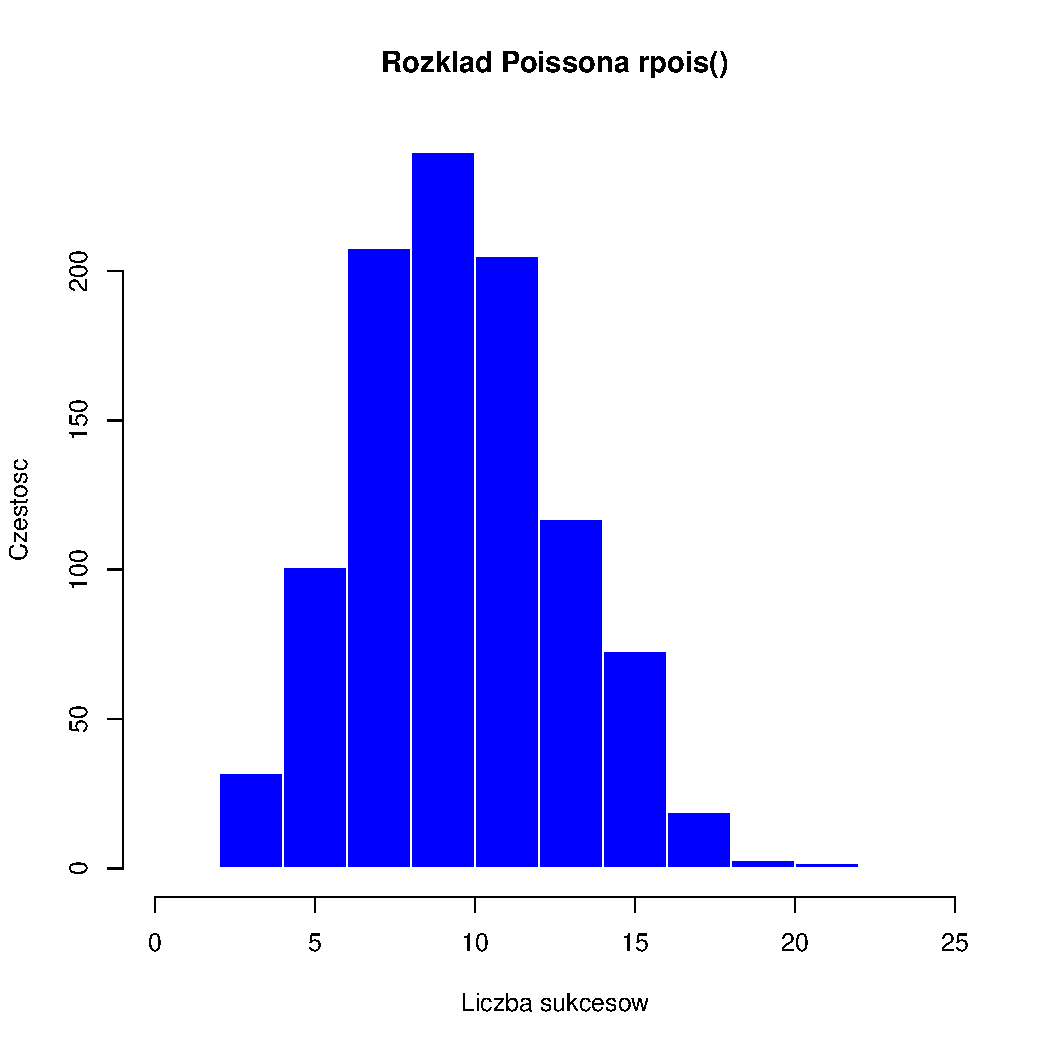
\includegraphics[width=\maxwidth]{figure/unnamed-chunk-10-2} 

}


\end{knitrout}


\end{itemize}

%%%%%%%%%%%%%%%%%%%%%%%%%%%%%%%%%%%%%%%%%%%%%%%%%%%%%%%%%%%%%%%%%%%%%%%%%%
%%%%%%%%%%%%%%%%%%%%%%%%%%%%%%%%%%%%%%%%%%%%%%%%%%%%%%%%%%%%%%%%%%%%%%%%%%
\end{document}
